%% 
%% Copyright 2007-2020 Elsevier Ltd
%% 
%% This file is part of the 'Elsarticle Bundle'.
%% ---------------------------------------------
%% 
%% It may be distributed under the conditions of the LaTeX Project Public
%% License, either version 1.2 of this license or (at your option) any
%% later version.  The latest version of this license is in
%%    http://www.latex-project.org/lppl.txt
%% and version 1.2 or later is part of all distributions of LaTeX
%% version 1999/12/01 or later.
%% 
%% The list of all files belonging to the 'Elsarticle Bundle' is
%% given in the file `manifest.txt'.
%% 
%% Template article for Elsevier's document class `elsarticle'
%% with harvard style bibliographic references

\documentclass[final,5p,times,twocolumn,authoryear]{elsarticle}

%% For including figures, graphicx.sty has been loaded in
%% elsarticle.cls. If you prefer to use the old commands
%% please give \usepackage{epsfig}

%% The amssymb package provides various useful mathematical symbols
\usepackage{hyperref}
\usepackage{amssymb}
\usepackage{lipsum}

%% The amsthm package provides extended theorem environments
%% \usepackage{amsthm}

%% The lineno packages adds line numbers. Start line numbering with
%% \begin{linenumbers}, end it with \end{linenumbers}. Or switch it on
%% for the whole article with \linenumbers.
%% \usepackage{lineno}

%% You might want to define your own abbreviated commands for common used terms, e.g.:
\newcommand{\kms}{km\,s$^{-1}$}
\newcommand{\msun}{$M_\odot}

\setcitestyle{square}

\begin{document}

\begin{frontmatter}

\title{OpenMPI implementation of Burrows-Wheeler Transform for substring matching applied to genomics}

\author{Andrei S. Blindu}
\affiliation{organization={University of Pavia, Computer Engineering},%Department and Organization
            city={Pavia},
            country={Italy}}

\begin{abstract}
%% Text of abstract
The aim of this project is to provide an efficient parallel implementation of a substring matching algorithm and apply it to the search of genes within the genome of an organism. After implementing the serial algorithm (using C/C++), an a priori study of the available parallelism has been conducted to identify the parts of the code that could be parallelized and then the code has been modified in order to run on multiple CPUs by using OpenMPI. The performance in terms of strong and weak scalability of the parallel implementation have been evaluated by running the code on Google Cloud Platform virtual instances in order to exploit the resources of a cluster of machines. A significant speedup has been obtained compared to the serial version, although under certain conditions the code is not able to scale efficiently as discussed later.
\end{abstract}

\begin{keyword}
Substring Matching \sep Genomics \sep Burrows-Wheeler Transform \sep Parallelization \sep Open MPI \sep Google Cloud Platform
\end{keyword}

\end{frontmatter}

% Table of contents
\tableofcontents

\vspace{\baselineskip}

%% main text

\section{Biological context and Data}
\label{Biological context and Data}
The algorithm considered in this project is being used to find a gene within the genome of an organism. The genome is made up of DNA and contains the set of genes of an organism which are responsible for its traits and characteristics.
DNA is a long double helix molecule composed by a sequence of nucleotides\cite{nucleotide}, each nucleotide is composed by deoxyribose sugar, a phosphate group and a nucleobase. There are four types of nucleobases in DNA: guanine (G), adenine (A), cytosine (C) and thymine (T).
In bioinformatics applications, the genome and the genes are usually considered as long strings of computer code composed by four possible letters (G,A,C,T). \\
The genomes used for this analysis have been taken from the NCBI website\cite{ncbi}. \\
Genomes of different sizes have been used in order to study how the performance changes with respect to the input dataset dimension:
\begin{itemize}
    \item \emph{Escherichia coli}, bacteria commonly found in the lower intestine of warm-blooded organisms\cite{ecoli}, 4.6MB \cite{ecoli dataset}
    \item \emph{Entamoeba invadens}, an amoebozoa parasite of reptiles\cite{entamoeba}, 40.9MB \cite{entamoeba dataset}
    \item \emph{Formica exsecta}, is a species of ant found from Western Europe to Asia \cite{formica}, 277.6MB \cite{formica dataset}
\end{itemize}


\section{Analysis of the serial algorithm}
Having efficient algorithms that allow us to deal with huge genetic sequences is crucial in the bioinformatics field. One of the most used algorithms is the Burrows-Wheeler Transform which was originally intended for data compression but it is used also for string pattern matching problems.

\subsection{Burrows-Wheeler Transform}
The Burrows-Wheeler Transform restructures the original string in a way that is more compressible. It does so by building a matrix whose rows are all the cyclic shifts of the input string, then the rows are lexicographically sorted and finally the last column is selected as the output of the BWT.
Let's consider the following example in Figure \ref{fig:bwt-label} taken from \cite{mreasy}.
\begin{figure}
    \centering
    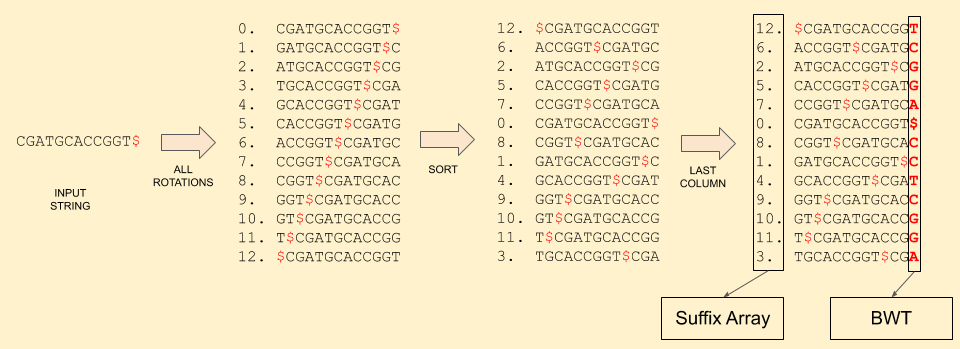
\includegraphics[width=1\textwidth]{images/bwt.png}
    \caption{Burrows-Wheeler Transform}
    \label{fig:bwt-label}
\end{figure}
\\ We take the last column because it can be proven that we can recover all the cyclic rotations rows from it and it is the only column having this property that is important to compute the inverse of the transform \cite{geeks}. Moreover, it has better symbol clustering, which means that the same symbols are often grouped together and this favours efficient compression \cite{geeks}. \\
The implementation\cite{bwt.h me} of the Burrows-Wheeler Transform presented for this project has been taken from \cite{geeks}.

\subsection{BWT pattern matching}


\section{A priori study of available parallelism}


\section{OpenMPI parallel implementation}


\section{Performance and scalability analysis}

\subsection{Fat cluster}
\subsubsection{Intra-regional}
\subsubsection{Infra-regional}

\subsection{Light cluster}
\subsubsection{Intra-regional}
\subsubsection{Infra-regional}


\section{Conclusions}

\begin{thebibliography}{9}
\bibitem{nucleotide} \url{https://en.wikipedia.org/wiki/Nucleotide}
\bibitem{ncbi} \url{https://www.ncbi.nlm.nih.gov/genbank/}
\bibitem{ecoli} \url{https://en.wikipedia.org/wiki/Escherichia_coli}
\bibitem{ecoli dataset} \url{https://www.ncbi.nlm.nih.gov/datasets/taxonomy/562/}
\bibitem{entamoeba} \url{https://en.wikipedia.org/wiki/Entamoeba_invadens}
\bibitem{entamoeba dataset} \url{https://www.ncbi.nlm.nih.gov/datasets/taxonomy/33085/}
\bibitem{formica} \url{https://en.wikipedia.org/wiki/Formica_exsecta}
\bibitem{formica dataset} \url{https://www.ncbi.nlm.nih.gov/datasets/taxonomy/72781/}
\bibitem{geeks}
\url{https://www.geeksforgeeks.org/burrows-wheeler-data-transform-algorithm/}
\bibitem{mreasy} 
\url{https://mr-easy.github.io/2019-12-19-burrows-wheeler-alignment-part-1/}
\bibitem{bwt.h me}
\url{https://github.com/AndreiBlindu/genome-pattern-search-OpenMPI/blob/main/src/utils/bwt.h}
\end{thebibliography}


\end{document}
